\subsubsection{Chua's Circuit}
 \begin{itemize}
  \item \textbf{Methodology}
We constructed the circuit using 4 TL082 I.C.'s and commercial resistors with the values used during simulation, Trimmer resistors to be able to move the resistor values of R.

            \begin{figure}[h]
            \centering
            \includegraphics[scale=0.1]{imagenes/2-benford/chua_breadboard.jpg}
            \caption{Chua's System Breadboard}
            \end{figure}
We used two oscilloscope probes to measure the voltage from the two capacitors, and did our measurements with  a Tektronix DS201 Oscilloscope with a direct method sampling.

 The first digit distribution was determined from the voltage measured at the terminals of C1,varying R from 1700$\Omega$ to 1900$\Omega$in $25\Omega$ intervals, values in which Chua's Circuit presented chaotic behaviour. The first digits (without leading zeroes) of the voltage values at discrete points were analyzed, the oscilloscope allowed us to take 2000 samples from a 250 $\mu$s period. We compared the first digit distribution of the dataset with the distribution given by Benford's Law using the Mean Absolute Deviation (MAD) proposed by \cite{Nigrini97}.



  \item \textbf{Results}
We put a table with the MAD results at each value of R:
\begin{center}
    \begin{tabular}{ c | c | c }
        R & MAD for VC1 & MAD forVC2\\
        1700 & 0.0266 & 0.0941\\ \hline
        1725 & 0.0308 & 0.0894\\ \hline
        1750 & 0.0225 & 0.0937\\ \hline
        1775 & 0.0213 & 0.0894\\ \hline
        1800 & 0.0515 & 0.0817\\ \hline
        1825 & 0.0620 & 0.0757\\ \hline
        1850 & 0.0801 & 0.0616\\ \hline
        1875 & 0.0864 & 0.0566\\ \hline
        1900 & 0.0848 & 0.0477\\ \hline


    \end{tabular}
\end{center}

The closest value to 0.015, obtained with R=1775 measuring $V_{C1}$
\begin{figure}[H]
    \centering
    \includegraphics[scale=0.4]{imagenes/2-benford/benford_chua1775.png}
    \caption{Benford's Law against VC1}
\end{figure}
\item \textbf{Remarks}

It was noticed that for R between 1730 and 1775, there is a more clear First Digit Distribution according to Benford's Law; however, the measurements did not comply with MAD's criterion which expects at most 0.015 in order to be compliant with Benford's Law. An additional measurement, with R=2000$\Omega$, was taken, value at which the system behaves as a quasi-periodic oscillator. It was noticed that the first digit distribution is more uniform.

\begin{figure}[H]
    \centering
    \begin{subfigure}[b]{0.4\textwidth}
        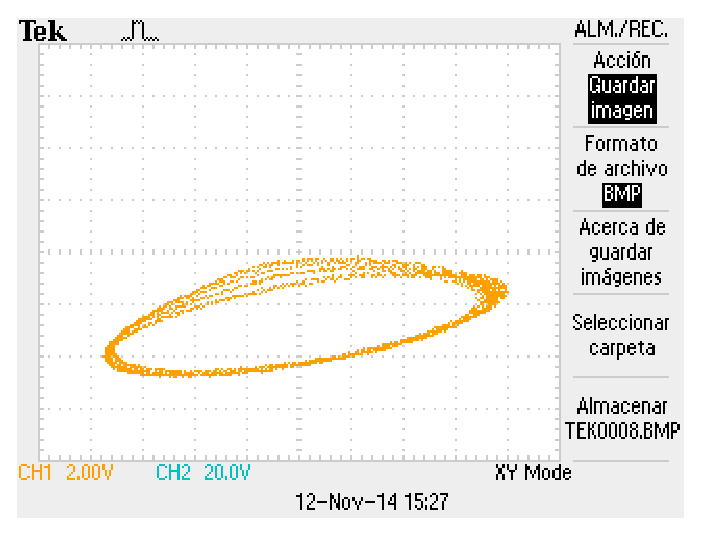
\includegraphics[width=\textwidth]{imagenes/2-benford/chua_2000.eps}
        \caption{V1-V2 $V_x$ vs $V_y$ plot}
    \end{subfigure}
    \begin{subfigure}[b]{0.8\textwidth}
        \includegraphics[width=\textwidth]{imagenes/2-benford/benford_chua20.png}
        \caption{Bifurcation Diagram varying b}
    \end{subfigure}
\end{figure}

\end{itemize}
\subsubsection{Takougang Circuit}
\begin{itemize}
    \item \textbf{Methodology} The circuit was connected using a standard breadboard, according to the diagram. All passive components had a nominal value equal to the ones proposed in the schematic, with a tolerance of 5\%. A regulated voltage source, set to $\pm$ 12 V was utilized to feed the active components which were the same as stated in the schematic. A third output of the regulated voltage source served to provide a stable input for the circuit ($V_b$). Later, a digital oscilloscope was used in order to obtain the data provided by the circuit.

    A 1 GHz band-width oscilloscope (Agilent DSO6104A) was chosen, and it was configured in order to reduce random noise. The sampler uses an averaging algorithm which delivers data with less noise, and reduces the vertical resolution (as low as 0.7 mV). With the data obtained from that oscilloscope the analysis was more reliable, and results confirmed what was expected from the simulations, although only 1000 samples in an interval of 10 ms were fetched.
    \begin{figure}[H]
        \centering
        \includegraphics[scale=0.4]{imagenes/2-benford/Tak_brd.png}
        \caption{Benford's Law against VC1}
    \end{figure}
    \item \textbf{Results}
    The first digit distribution of the voltages was taken following the same methodology as with Chua's System, values of $V_b$ were changed and the value of the MAD was obtained from each distribution.
    \begin{center}
        \begin{tabular}{ c | c | c }
            \hline
            $V_b$  & $MAD for V_x$&$ MAD for V_y$\\ \hline
            82mV  & 0.0775 & 0.0607 \\ \hline
            92mV  & 0.0789 & 0.0621 \\ \hline
            102mv & 0.0779 & 0.0620  \\ \hline
            112mv & 0.0722 & 0.0586  \\ \hline
            117mv & 0.0731 & 0.0565  \\ \hline
            122mv & 0.0761 & 0.0607  \\ \hline
            127mv & 0.0702 & 0.0581  \\ \hline
            132mv & 0.0726 & 0.0568  \\ \hline
            137mv & 0.0723 & 0.0588  \\ \hline
            142mv & 0.0689 & 0.0566  \\ \hline
            147mv & 0.0649 & 0.0492  \\ \hline
            152mv & 0.0689 & 0.0540  \\ \hline
            157mv & 0.0712 & 0.0556   \\ \hline
            167mv & 0.0713 & 0.0546  \\ \hline
            187mv & 0.0642 & 0.0499  \\ \hline
            197mv & 0.0619 & 0.0492  \\ \hline
            217mv & 0.0644 & 0.0521  \\ \hline
            237mv & 0.0574 & 0.0515  \\ \hline
            257mv & 0.0552 & 0.0514  \\ \hline
            277mv & 0.0464 & 0.0450  \\ \hline
            112mv (H-Res) & 0.0126 & 0.0149  \\ \hline
            132mv  (H-Res)& 0.0114 & 0.0056  \\ \hline
            152mv  (H-Res)& 0.0106 & 0.0143  \\ \hline
            172mv  (H-Res)& 0.0077 & 0.0118  \\ \hline
            192mv  (H-Res)& 0.0080 & 0.0121  \\ \hline

        \end{tabular}
    \end{center}

We notice we have the best agreement with Benford's Law with $V_b=132mV$ Which gives a MAD value of 0.0056

            \begin{figure}[h]
            \centering
            \includegraphics[scale=0.4]{imagenes/2-benford/benford_shilnikov_1.png}
            \caption{Benford's Law against digit distribution of $V_y$}
            \end{figure}

  \item \textbf{Remarks}

Simulations from Simulink gave a better accordance with $V_b=132mV$, however measuring without High-resolution sampling we did not obtain proper distributions, until we activated that sampling method, we got a distribution according to Benford's Law
 \end{itemize}
